\batchmode
\documentclass[12pt,twoside]{article}
\RequirePackage{ifthen}


\usepackage{healpix,html,graphicx,makeidx,color,apalike} 
%
\renewcommand{\ell}{l}
\sloppy



\pagecolor[gray]{.7}

\usepackage[latin1]{inputenc}



\makeatletter

\makeatletter
\count@=\the\catcode`\_ \catcode`\_=8 
\newenvironment{tex2html_wrap}{}{}%
\catcode`\<=12\catcode`\_=\count@
\newcommand{\providedcommand}[1]{\expandafter\providecommand\csname #1\endcsname}%
\newcommand{\renewedcommand}[1]{\expandafter\providecommand\csname #1\endcsname{}%
  \expandafter\renewcommand\csname #1\endcsname}%
\newcommand{\newedenvironment}[1]{\newenvironment{#1}{}{}\renewenvironment{#1}}%
\let\newedcommand\renewedcommand
\let\renewedenvironment\newedenvironment
\makeatother
\let\mathon=$
\let\mathoff=$
\ifx\AtBeginDocument\undefined \newcommand{\AtBeginDocument}[1]{}\fi
\newbox\sizebox
\setlength{\hoffset}{0pt}\setlength{\voffset}{0pt}
\addtolength{\textheight}{\footskip}\setlength{\footskip}{0pt}
\addtolength{\textheight}{\topmargin}\setlength{\topmargin}{0pt}
\addtolength{\textheight}{\headheight}\setlength{\headheight}{0pt}
\addtolength{\textheight}{\headsep}\setlength{\headsep}{0pt}
\setlength{\textwidth}{349pt}
\newwrite\lthtmlwrite
\makeatletter
\let\realnormalsize=\normalsize
\global\topskip=2sp
\def\preveqno{}\let\real@float=\@float \let\realend@float=\end@float
\def\@float{\let\@savefreelist\@freelist\real@float}
\def\liih@math{\ifmmode$\else\bad@math\fi}
\def\end@float{\realend@float\global\let\@freelist\@savefreelist}
\let\real@dbflt=\@dbflt \let\end@dblfloat=\end@float
\let\@largefloatcheck=\relax
\let\if@boxedmulticols=\iftrue
\def\@dbflt{\let\@savefreelist\@freelist\real@dbflt}
\def\adjustnormalsize{\def\normalsize{\mathsurround=0pt \realnormalsize
 \parindent=0pt\abovedisplayskip=0pt\belowdisplayskip=0pt}%
 \def\phantompar{\csname par\endcsname}\normalsize}%
\def\lthtmltypeout#1{{\let\protect\string \immediate\write\lthtmlwrite{#1}}}%
\newcommand\lthtmlhboxmathA{\adjustnormalsize\setbox\sizebox=\hbox\bgroup\kern.05em }%
\newcommand\lthtmlhboxmathB{\adjustnormalsize\setbox\sizebox=\hbox to\hsize\bgroup\hfill }%
\newcommand\lthtmlvboxmathA{\adjustnormalsize\setbox\sizebox=\vbox\bgroup %
 \let\ifinner=\iffalse \let\)\liih@math }%
\newcommand\lthtmlboxmathZ{\@next\next\@currlist{}{\def\next{\voidb@x}}%
 \expandafter\box\next\egroup}%
\newcommand\lthtmlmathtype[1]{\gdef\lthtmlmathenv{#1}}%
\newcommand\lthtmllogmath{\dimen0\ht\sizebox \advance\dimen0\dp\sizebox
  \ifdim\dimen0>.95\vsize
   \lthtmltypeout{%
*** image for \lthtmlmathenv\space is too tall at \the\dimen0, reducing to .95 vsize ***}%
   \ht\sizebox.95\vsize \dp\sizebox\z@ \fi
  \lthtmltypeout{l2hSize %
:\lthtmlmathenv:\the\ht\sizebox::\the\dp\sizebox::\the\wd\sizebox.\preveqno}}%
\newcommand\lthtmlfigureA[1]{\let\@savefreelist\@freelist
       \lthtmlmathtype{#1}\lthtmlvboxmathA}%
\newcommand\lthtmlpictureA{\bgroup\catcode`\_=8 \lthtmlpictureB}%
\newcommand\lthtmlpictureB[1]{\lthtmlmathtype{#1}\egroup
       \let\@savefreelist\@freelist \lthtmlhboxmathB}%
\newcommand\lthtmlpictureZ[1]{\hfill\lthtmlfigureZ}%
\newcommand\lthtmlfigureZ{\lthtmlboxmathZ\lthtmllogmath\copy\sizebox
       \global\let\@freelist\@savefreelist}%
\newcommand\lthtmldisplayA{\bgroup\catcode`\_=8 \lthtmldisplayAi}%
\newcommand\lthtmldisplayAi[1]{\lthtmlmathtype{#1}\egroup\lthtmlvboxmathA}%
\newcommand\lthtmldisplayB[1]{\edef\preveqno{(\theequation)}%
  \lthtmldisplayA{#1}\let\@eqnnum\relax}%
\newcommand\lthtmldisplayZ{\lthtmlboxmathZ\lthtmllogmath\lthtmlsetmath}%
\newcommand\lthtmlinlinemathA{\bgroup\catcode`\_=8 \lthtmlinlinemathB}
\newcommand\lthtmlinlinemathB[1]{\lthtmlmathtype{#1}\egroup\lthtmlhboxmathA
  \vrule height1.5ex width0pt }%
\newcommand\lthtmlinlineA{\bgroup\catcode`\_=8 \lthtmlinlineB}%
\newcommand\lthtmlinlineB[1]{\lthtmlmathtype{#1}\egroup\lthtmlhboxmathA}%
\newcommand\lthtmlinlineZ{\egroup\expandafter\ifdim\dp\sizebox>0pt %
  \expandafter\centerinlinemath\fi\lthtmllogmath\lthtmlsetinline}
\newcommand\lthtmlinlinemathZ{\egroup\expandafter\ifdim\dp\sizebox>0pt %
  \expandafter\centerinlinemath\fi\lthtmllogmath\lthtmlsetmath}
\newcommand\lthtmlindisplaymathZ{\egroup %
  \centerinlinemath\lthtmllogmath\lthtmlsetmath}
\def\lthtmlsetinline{\hbox{\vrule width.1em \vtop{\vbox{%
  \kern.1em\copy\sizebox}\ifdim\dp\sizebox>0pt\kern.1em\else\kern.3pt\fi
  \ifdim\hsize>\wd\sizebox \hrule depth1pt\fi}}}
\def\lthtmlsetmath{\hbox{\vrule width.1em\kern-.05em\vtop{\vbox{%
  \kern.1em\kern0.8 pt\hbox{\hglue.17em\copy\sizebox\hglue0.8 pt}}\kern.3pt%
  \ifdim\dp\sizebox>0pt\kern.1em\fi \kern0.8 pt%
  \ifdim\hsize>\wd\sizebox \hrule depth1pt\fi}}}
\def\centerinlinemath{%
  \dimen1=\ifdim\ht\sizebox<\dp\sizebox \dp\sizebox\else\ht\sizebox\fi
  \advance\dimen1by.5pt \vrule width0pt height\dimen1 depth\dimen1 
 \dp\sizebox=\dimen1\ht\sizebox=\dimen1\relax}

\def\lthtmlcheckvsize{\ifdim\ht\sizebox<\vsize 
  \ifdim\wd\sizebox<\hsize\expandafter\hfill\fi \expandafter\vfill
  \else\expandafter\vss\fi}%
\providecommand{\selectlanguage}[1]{}%
\makeatletter \tracingstats = 1 


\begin{document}
\pagestyle{empty}\thispagestyle{empty}\lthtmltypeout{}%
\lthtmltypeout{latex2htmlLength hsize=\the\hsize}\lthtmltypeout{}%
\lthtmltypeout{latex2htmlLength vsize=\the\vsize}\lthtmltypeout{}%
\lthtmltypeout{latex2htmlLength hoffset=\the\hoffset}\lthtmltypeout{}%
\lthtmltypeout{latex2htmlLength voffset=\the\voffset}\lthtmltypeout{}%
\lthtmltypeout{latex2htmlLength topmargin=\the\topmargin}\lthtmltypeout{}%
\lthtmltypeout{latex2htmlLength topskip=\the\topskip}\lthtmltypeout{}%
\lthtmltypeout{latex2htmlLength headheight=\the\headheight}\lthtmltypeout{}%
\lthtmltypeout{latex2htmlLength headsep=\the\headsep}\lthtmltypeout{}%
\lthtmltypeout{latex2htmlLength parskip=\the\parskip}\lthtmltypeout{}%
\lthtmltypeout{latex2htmlLength oddsidemargin=\the\oddsidemargin}\lthtmltypeout{}%
\makeatletter
\if@twoside\lthtmltypeout{latex2htmlLength evensidemargin=\the\evensidemargin}%
\else\lthtmltypeout{latex2htmlLength evensidemargin=\the\oddsidemargin}\fi%
\lthtmltypeout{}%
\makeatother
\setcounter{page}{1}
\onecolumn

% !!! IMAGES START HERE !!!

\stepcounter{section}
{\newpage\clearpage
\lthtmlinlinemathA{tex2html_wrap_inline1113}%
$\sim 10^6$%
\lthtmlinlinemathZ
\lthtmlcheckvsize\clearpage}

{\newpage\clearpage
\lthtmlinlinemathA{tex2html_wrap_inline1115}%
$\lq$%
\lthtmlinlinemathZ
\lthtmlcheckvsize\clearpage}

{\newpage\clearpage
\lthtmlinlinemathA{tex2html_wrap_inline1117}%
$7^\circ$%
\lthtmlinlinemathZ
\lthtmlcheckvsize\clearpage}

{\newpage\clearpage
\lthtmlinlinemathA{tex2html_wrap_inline1119}%
$\sim 10'$%
\lthtmlinlinemathZ
\lthtmlcheckvsize\clearpage}

{\newpage\clearpage
\lthtmlinlinemathA{tex2html_wrap_inline1121}%
$N_{pix}\sim $%
\lthtmlinlinemathZ
\lthtmlcheckvsize\clearpage}

{\newpage\clearpage
\lthtmlinlinemathA{tex2html_wrap_inline1123}%
$\times 1.5\, 10^6$%
\lthtmlinlinemathZ
\lthtmlcheckvsize\clearpage}

\stepcounter{section}
{\newpage\clearpage
\lthtmlfigureA{figure30}%
\begin{figure}\centerline{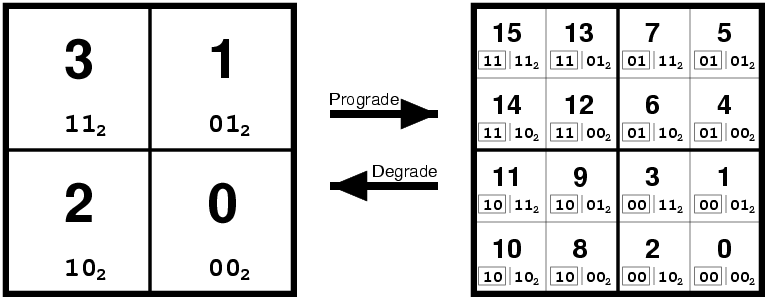
\includegraphics[bb=1pt 1pt 768pt 300pt,width=0.9\textwidth]{fig/quad_tree}\htmlimage{}}
\par

\end{figure}%
\lthtmlfigureZ
\lthtmlcheckvsize\clearpage}

{\newpage\clearpage
\lthtmlinlinemathA{tex2html_wrap_inline1127}%
$N_{side} = \,1,\,2,\,4,\,8$%
\lthtmlinlinemathZ
\lthtmlcheckvsize\clearpage}

{\newpage\clearpage
\lthtmlinlinemathA{tex2html_wrap_inline1129}%
$N_{pix} = 12 \times N_{side}^2 = \,12,\,48,\,192,\,768$%
\lthtmlinlinemathZ
\lthtmlcheckvsize\clearpage}

{\newpage\clearpage
\lthtmlfigureA{figure51}%
\begin{figure}\centerline{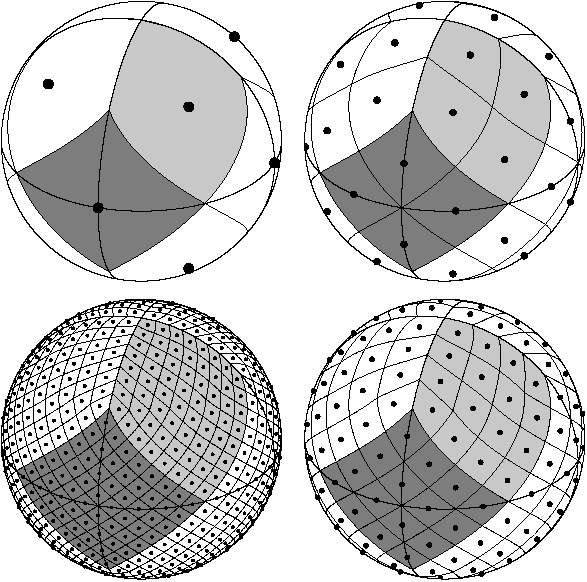
\includegraphics[bb=1pt 1pt 587pt 800pt,width=8cm]{fig/introf1}\htmlimage{}}
\par

\end{figure}%
\lthtmlfigureZ
\lthtmlcheckvsize\clearpage}

\stepcounter{section}
{\newpage\clearpage
\lthtmlinlinemathA{tex2html_wrap_inline1139}%
$\cos \theta = a \pm b \cdot \phi\htmlimage{}$%
\lthtmlinlinemathZ
\lthtmlcheckvsize\clearpage}

{\newpage\clearpage
\lthtmlinlinemathA{tex2html_wrap_inline1141}%
$\cos \theta = a + b / \phi^2\htmlimage{}$%
\lthtmlinlinemathZ
\lthtmlcheckvsize\clearpage}

{\newpage\clearpage
\lthtmlinlinemathA{tex2html_wrap_inline1143}%
$\cos \theta = a + b / (\pi/2 - \phi) ^2\htmlimage{}$%
\lthtmlinlinemathZ
\lthtmlcheckvsize\clearpage}

{\newpage\clearpage
\lthtmlfigureA{figure70}%
\begin{figure}\centerline{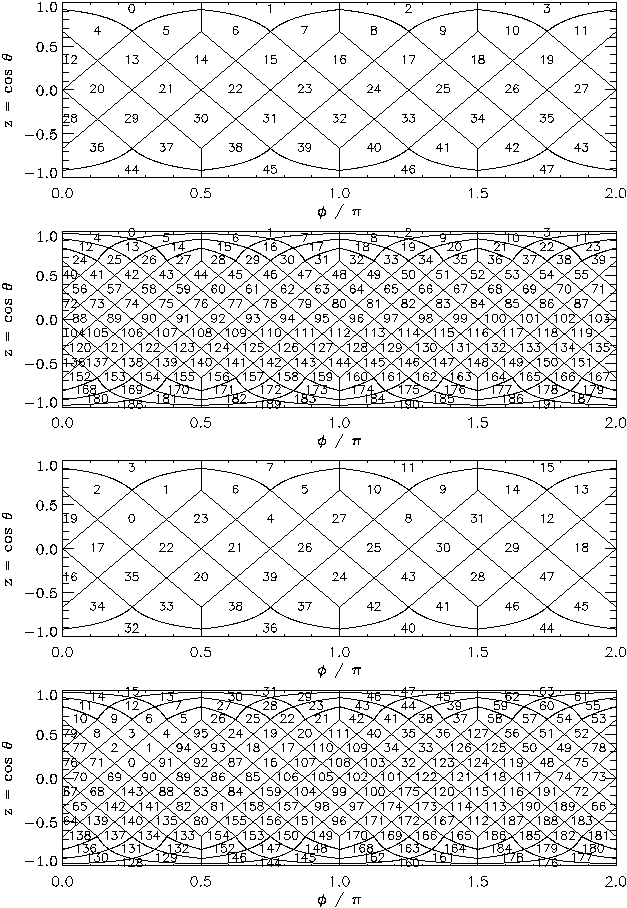
\includegraphics[bb=1pt 1pt 627pt
    908pt,width=15cm]{fig/introf2}\htmlimage{}}
\par

\end{figure}%
\lthtmlfigureZ
\lthtmlcheckvsize\clearpage}

\stepcounter{section}
\appendix
\stepcounter{section}
{\newpage\clearpage
\lthtmldisplayA{eqnarray109}%
\begin{eqnarray}
  f({ \gamma})&=&\sum_{l=0}^{l_{max}}\sum_{m}a_{lm}Y_{lm}(\gamma),\htmlimage{}
\end{eqnarray}%
\lthtmldisplayZ
\lthtmlcheckvsize\clearpage}

{\newpage\clearpage
\lthtmlinlinemathA{tex2html_wrap_inline1159}%
${{\gamma}}$%
\lthtmlinlinemathZ
\lthtmlcheckvsize\clearpage}

{\newpage\clearpage
\lthtmlinlinemathA{tex2html_wrap_inline1161}%
$\theta\in[0,\pi]$%
\lthtmlinlinemathZ
\lthtmlcheckvsize\clearpage}

{\newpage\clearpage
\lthtmlinlinemathA{tex2html_wrap_inline1163}%
$\phi\in[0,2\pi)$%
\lthtmlinlinemathZ
\lthtmlcheckvsize\clearpage}

{\newpage\clearpage
\lthtmlinlinemathA{tex2html_wrap_inline1179}%
$f({ \gamma})$%
\lthtmlinlinemathZ
\lthtmlcheckvsize\clearpage}

{\newpage\clearpage
\lthtmlinlinemathA{tex2html_wrap_inline1181}%
$N_{\rm {pix}}$%
\lthtmlinlinemathZ
\lthtmlcheckvsize\clearpage}

{\newpage\clearpage
\lthtmlinlinemathA{tex2html_wrap_inline1183}%
$\gamma_{p}$%
\lthtmlinlinemathZ
\lthtmlcheckvsize\clearpage}

{\newpage\clearpage
\lthtmlinlinemathA{tex2html_wrap_inline1185}%
$p\in[0,N_{\rm {pix}}-1]$%
\lthtmlinlinemathZ
\lthtmlcheckvsize\clearpage}

{\newpage\clearpage
\lthtmldisplayA{eqnarray131}%
\begin{eqnarray}
  \hat{a}_{lm}&=& \frac{4\pi}{N_{\rm {pix}}}\sum_{p=0}^{N_{\rm {pix}}-1}
  Y^\ast_{lm}(\gamma_p) f(\gamma_p),\htmlimage{}
\end{eqnarray}%
\lthtmldisplayZ
\lthtmlcheckvsize\clearpage}

\stepcounter{subsection}
{\newpage\clearpage
\lthtmlinlinemathA{tex2html_wrap_inline1191}%
$\hat{a}_{lm}$%
\lthtmlinlinemathZ
\lthtmlcheckvsize\clearpage}

{\newpage\clearpage
\lthtmlinlinemathA{tex2html_wrap_inline1193}%
$\hat{C}_l$%
\lthtmlinlinemathZ
\lthtmlcheckvsize\clearpage}

{\newpage\clearpage
\lthtmldisplayA{eqnarray148}%
\begin{eqnarray}
  \hat{C}_l&=&\frac{1}{2l +1}\sum_{m} \vert\hat{a}_{lm}\vert^2.\htmlimage{}
\end{eqnarray}%
\lthtmldisplayZ
\lthtmlcheckvsize\clearpage}

{\newpage\clearpage
\lthtmlinlinemathA{tex2html_wrap_inline1197}%
$f(\gamma_p)$%
\lthtmlinlinemathZ
\lthtmlcheckvsize\clearpage}

{\newpage\clearpage
\lthtmlinlinemathA{tex2html_wrap_inline1207}%
$f(\gamma)/\sqrt{4 \pi}$%
\lthtmlinlinemathZ
\lthtmlcheckvsize\clearpage}

{\newpage\clearpage
\lthtmlinlinemathA{tex2html_wrap_inline1213}%
$1/(4\pi)$%
\lthtmlinlinemathZ
\lthtmlcheckvsize\clearpage}

{\newpage\clearpage
\lthtmlinlinemathA{tex2html_wrap_inline1215}%
$f(\gamma)$%
\lthtmlinlinemathZ
\lthtmlcheckvsize\clearpage}

{\newpage\clearpage
\lthtmlinlinemathA{tex2html_wrap_inline1217}%
$4\pi$%
\lthtmlinlinemathZ
\lthtmlcheckvsize\clearpage}

{\newpage\clearpage
\lthtmlinlinemathA{tex2html_wrap_inline1233}%
$\Delta T/T $%
\lthtmlinlinemathZ
\lthtmlcheckvsize\clearpage}

{\newpage\clearpage
\lthtmlinlinemathA{tex2html_wrap_inline1235}%
$\Delta T$%
\lthtmlinlinemathZ
\lthtmlcheckvsize\clearpage}

{\newpage\clearpage
\lthtmlinlinemathA{tex2html_wrap_inline1237}%
$\mu K$%
\lthtmlinlinemathZ
\lthtmlcheckvsize\clearpage}

\stepcounter{subsection}
{\newpage\clearpage
\lthtmldisplayA{eqnarray174}%
\begin{eqnarray}
  D_{X,l}&=&\frac{l(l+1)}{(2\pi)T_{CMB}^2}C_{X,l},\htmlimage{}
\end{eqnarray}%
\lthtmldisplayZ
\lthtmlcheckvsize\clearpage}

\stepcounter{subsection}

%
\providecommand{\Cl}[1]{C_{l}^{\rm #1}}%


%
\providecommand{\Chl}[1]{C_{l}^{\rm{#1}}}%


%
\providecommand{\Czl}[1]{C_{\rm{#1},l}}%


%
\providecommand{\alm}[1]{a_{lm}^{\rm #1}}%


%
\providecommand{\azlm}[1]{a_{{\rm #1},lm}}%


%
\providecommand{\pushup}{\rule[.3cm]{0cm}{.2cm}}%


%
\providecommand{\pushdn}{\rule[-.3cm]{0cm}{.2cm}}%


%
\providecommand{\push}{\rule[.3cm]{0cm}{.2cm}\rule[-.3cm]{0cm}{.2cm}}%


%
\providecommand{\vecn}{{\bf n}}%


%
\providecommand{\veceo}{{\bf{e}_{1}}}%


%
\providecommand{\vecet}{{\bf{e}_{2}}}%


%
\providecommand{\vectheta}{{\bf{e}_\theta}}%


%
\providecommand{\vecphi}{{\bf{e}_\phi}}%


%
\providecommand{\mattwo}[2]{{
\left( 
\begin{array}{c} #1 \rule[.3cm]{0cm}{.2cm}\rule[-.3cm]{0cm}{.2cm}\\#2 \rule[.3cm]{0cm}{.2cm}\rule[-.3cm]{0cm}{.2cm}\end{array}
\right) 
}}%

{\newpage\clearpage
\lthtmlfigureA{figure230}%
\begin{figure}\centerline{\includegraphics[bb=1pt 1pt 800pt 792pt,width=6in]{fig/plot_orthpol2}\htmlimage{}}
\par

\end{figure}%
\lthtmlfigureZ
\lthtmlcheckvsize\clearpage}

\stepcounter{subsubsection}
{\newpage\clearpage
\lthtmlinlinemathA{tex2html_wrap_inline1255}%
$2\, \times \, 2$%
\lthtmlinlinemathZ
\lthtmlcheckvsize\clearpage}

{\newpage\clearpage
\lthtmlinlinemathA{tex2html_wrap_inline1275}%
${\bf n}$%
\lthtmlinlinemathZ
\lthtmlcheckvsize\clearpage}

{\newpage\clearpage
\lthtmlinlinemathA{tex2html_wrap_inline1277}%
$({\bf {e}_{1}}, {\bf {e}_{2}})$%
\lthtmlinlinemathZ
\lthtmlcheckvsize\clearpage}

{\newpage\clearpage
\lthtmlinlinemathA{tex2html_wrap_inline1285}%
$\psi$%
\lthtmlinlinemathZ
\lthtmlcheckvsize\clearpage}

{\newpage\clearpage
\lthtmlinlinemathA{tex2html_wrap_inline1287}%
${{\bf {e}_{1}}}^{\prime}=\cos \psi \ {{\bf {e}_{1}}}+\sin\psi \ {{\bf {e}_{2}}}\htmlimage{}$%
\lthtmlinlinemathZ
\lthtmlcheckvsize\clearpage}

{\newpage\clearpage
\lthtmlinlinemathA{tex2html_wrap_inline1289}%
${{\bf {e}_{2}}}^{\prime}=-\sin \psi \ {{\bf {e}_{1}}}+\cos\psi \ {{\bf {e}_{2}}}\htmlimage{}$%
\lthtmlinlinemathZ
\lthtmlcheckvsize\clearpage}

{\newpage\clearpage
\lthtmldisplayA{eqnarray264}%
\begin{eqnarray}
  Q^{\prime}&=&\cos 2\psi \  Q + \sin 2\psi \ U \nonumber \htmlimage{} \\
  U^{\prime}&=&-\sin 2\psi \ Q + \cos 2\psi \ U     \htmlimage{}  
\end{eqnarray}%
\lthtmldisplayZ
\lthtmlcheckvsize\clearpage}

{\newpage\clearpage
\lthtmlinlinemathA{tex2html_wrap_inline1291}%
$Q\pm iU$%
\lthtmlinlinemathZ
\lthtmlcheckvsize\clearpage}

{\newpage\clearpage
\lthtmlinlinemathA{tex2html_wrap_inline1293}%
$\pm 2$%
\lthtmlinlinemathZ
\lthtmlcheckvsize\clearpage}

{\newpage\clearpage
\lthtmlinlinemathA{tex2html_wrap_inline1295}%
$\, _{\pm2}Y_l^m$%
\lthtmlinlinemathZ
\lthtmlcheckvsize\clearpage}

{\newpage\clearpage
\lthtmldisplayA{eqnarray275}%
\begin{eqnarray}
  T({\bf n})&=&\sum_{lm} a_{T,lm} Y_{lm}({\bf n}) \nonumber \\
  (Q+iU)({\bf n})&=&\sum_{lm} 
  a_{2,lm}\;_2Y_{lm}({\bf n}) \nonumber \htmlimage{} \\
  (Q-iU)({\bf n})&=&\sum_{lm}
  a_{-2,lm}\;_{-2}Y_{lm}({\bf n}).
  \htmlimage{}   
\end{eqnarray}%
\lthtmldisplayZ
\lthtmlcheckvsize\clearpage}

{\newpage\clearpage
\lthtmlinlinemathA{tex2html_wrap_inline1301}%
$({\bf {e}_{1}}, {\bf {e}_{2}})=({\bf {e}_\theta}, {\bf {e}_\phi})$%
\lthtmlinlinemathZ
\lthtmlcheckvsize\clearpage}

{\newpage\clearpage
\lthtmlinlinemathA{tex2html_wrap_inline1303}%
${\bf {e}_\theta}$%
\lthtmlinlinemathZ
\lthtmlcheckvsize\clearpage}

{\newpage\clearpage
\lthtmlinlinemathA{tex2html_wrap_inline1305}%
${\bf {e}_\phi}$%
\lthtmlinlinemathZ
\lthtmlcheckvsize\clearpage}

{\newpage\clearpage
\lthtmlinlinemathA{tex2html_wrap_inline1307}%
$_{\pm 2}a_{lm}$%
\lthtmlinlinemathZ
\lthtmlcheckvsize\clearpage}

{\newpage\clearpage
\lthtmldisplayA{eqnarray299}%
\begin{eqnarray}
a_{E,lm}&=&-(a_{2,lm}+a_{-2,lm})/2  \nonumber \htmlimage{} \\
a_{B,lm}&=&-(a_{2,lm}-a_{-2,lm})/2i, \htmlimage{}
\end{eqnarray}%
\lthtmldisplayZ
\lthtmlcheckvsize\clearpage}

{\newpage\clearpage
\lthtmldisplayA{eqnarray309}%
\begin{eqnarray}
  \langle a_{X,lm}^{*}
  a_{X,lm^\prime}\rangle &=& \delta_{m,m^\prime}C_{Xl}
  \quad
  \langle a_{T,lm}^{*}a_{E,lm}\rangle=\delta_{m,m^\prime}C_{Cl},\htmlimage{}
\end{eqnarray}%
\lthtmldisplayZ
\lthtmlcheckvsize\clearpage}

{\newpage\clearpage
\lthtmlinlinemathA{tex2html_wrap_inline1331}%
$\langle\cdots \rangle$%
\lthtmlinlinemathZ
\lthtmlcheckvsize\clearpage}

{\newpage\clearpage
\lthtmlinlinemathA{tex2html_wrap_inline1333}%
$\delta_{i,j}$%
\lthtmlinlinemathZ
\lthtmlcheckvsize\clearpage}

{\newpage\clearpage
\lthtmldisplayA{eqnarray325}%
\begin{eqnarray}
T({\bf n})&=&\sum_{lm} a_{T,lm} Y_{lm}({\bf n}) \nonumber \\
Q({\bf n})&=&-\sum_{lm} 
a_{E,lm} X_{1,lm} 
+i a_{B,lm}X_{2,lm} \nonumber \\
U({\bf n})&=&-\sum_{lm} 
a_{B,lm} X_{1,lm}-i a_{E,lm} X_{2,lm}
\htmlimage{}
\end{eqnarray}%
\lthtmldisplayZ
\lthtmlcheckvsize\clearpage}

{\newpage\clearpage
\lthtmlinlinemathA{tex2html_wrap_inline1335}%
$X_{1,lm}({\bf n})=(\;_2Y_{lm}+\;_{-2}Y_{lm})/2$%
\lthtmlinlinemathZ
\lthtmlcheckvsize\clearpage}

{\newpage\clearpage
\lthtmlinlinemathA{tex2html_wrap_inline1337}%
$X_{2,lm}({\bf n})=(\;_2Y_{lm}-\;_{-2}Y_{lm})/ 2$%
\lthtmlinlinemathZ
\lthtmlcheckvsize\clearpage}

{\newpage\clearpage
\lthtmlinlinemathA{tex2html_wrap_inline1357}%
$X_{1,lm}({\bf n})$%
\lthtmlinlinemathZ
\lthtmlcheckvsize\clearpage}

{\newpage\clearpage
\lthtmlinlinemathA{tex2html_wrap_inline1359}%
$X_{2,lm}({\bf n})$%
\lthtmlinlinemathZ
\lthtmlcheckvsize\clearpage}

{\newpage\clearpage
\lthtmlinlinemathA{tex2html_wrap_inline1361}%
$\htmlimage{} {X_{1,lm}({\bf n})=\sqrt{(2l+1) / 4\pi} F_{1,lm}(\theta)\ e^{im\phi}}$%
\lthtmlinlinemathZ
\lthtmlcheckvsize\clearpage}

{\newpage\clearpage
\lthtmlinlinemathA{tex2html_wrap_inline1363}%
$\htmlimage{} {X_{2,lm}({\bf n})=\sqrt{(2l+1) / 4\pi} F_{2,lm}(\theta)\ e^{im\phi}}$%
\lthtmlinlinemathZ
\lthtmlcheckvsize\clearpage}

{\newpage\clearpage
\lthtmlinlinemathA{tex2html_wrap_inline1365}%
$\htmlimage{} {F_{(1,2),lm}(\theta)}$%
\lthtmlinlinemathZ
\lthtmlcheckvsize\clearpage}

{\newpage\clearpage
\lthtmldisplayA{eqnarray390}%
\begin{eqnarray}
F_{1,lm}(\theta)&=&  N_{lm}
\left[ -\left({l-m^2 \over \sin^2\theta} 
+{1 \over 2}l(l-1)\right)P_l^m(\cos \theta)
+(l+m) {\cos \theta \over \sin^2 \theta} 
P_{l-1}^m(\cos\theta)\right] \nonumber \\
F_{2,lm}(\theta)&=&  N_{lm}{m \over
\sin^2 \theta}
[ -(l-1)\cos \theta P_l^m(\cos \theta)+(l+m) P_{l-1}^m(\cos\theta)], \htmlimage{}
\end{eqnarray}%
\lthtmldisplayZ
\lthtmlcheckvsize\clearpage}

{\newpage\clearpage
\lthtmldisplayA{eqnarray404}%
\begin{eqnarray}
   N_{lm}(\theta)&=& 2 \sqrt{(l-2)!(l-m)! \over (l+2)!(l+m)!}.\htmlimage{}
\end{eqnarray}%
\lthtmldisplayZ
\lthtmlcheckvsize\clearpage}

{\newpage\clearpage
\lthtmlinlinemathA{tex2html_wrap_inline1367}%
$F_{2,lm}(\theta)=0$%
\lthtmlinlinemathZ
\lthtmlcheckvsize\clearpage}

{\newpage\clearpage
\lthtmlinlinemathA{tex2html_wrap_inline1371}%
$\beta$%
\lthtmlinlinemathZ
\lthtmlcheckvsize\clearpage}

{\newpage\clearpage
\lthtmlinlinemathA{tex2html_wrap_inline1373}%
${\bf {e}_{1}}$%
\lthtmlinlinemathZ
\lthtmlcheckvsize\clearpage}

{\newpage\clearpage
\lthtmlinlinemathA{tex2html_wrap_inline1375}%
${\bf {e}_{2}}$%
\lthtmlinlinemathZ
\lthtmlcheckvsize\clearpage}

{\newpage\clearpage
\lthtmldisplayA{eqnarray414}%
\begin{eqnarray}
\sum_m \;_{s_1} Y_{lm}^*({\bf n}_1) 
\;_{s_2} Y_{lm}({\bf n}_2)&=&\sqrt{2l+1 \over 4 \pi} 
\;_{s_2} Y_{l-s_1}(\beta,\psi_1)e^{-is_2\psi_2} \htmlimage{}
\end{eqnarray}%
\lthtmldisplayZ
\lthtmlcheckvsize\clearpage}

{\newpage\clearpage
\lthtmldisplayA{eqnarray429}%
\begin{eqnarray}
\langle T_1T_2 \rangle&=&\sum_l {2l+1 \over 4 \pi}
C_{Tl} P_l(\cos \beta) \nonumber \\
\langle Q_{r}(1)Q_{r}(2) \rangle&=&\sum_l {2l+1 \over 4 \pi} [C_{El}
F_{1,l2}(\beta)-C_{Bl} F_{2,l2}(\beta)]  \nonumber \\
\langle U_{r}(1)U_{r}(2) \rangle&=&\sum_l {2l+1 \over 4 \pi}
[C_{Bl} F_{1,l2}(\beta)-C_{El} F_{2,l2}(\beta) ] \nonumber \\
\langle T(1)Q_{r}(2) 
\rangle&=& - \sum_l {2l+1 \over 4 \pi} C_{Cl} F_{1,l0}(\beta)\nonumber \\
\langle T(1)U_{r}(2) \rangle&=&0.\htmlimage{}
\end{eqnarray}%
\lthtmldisplayZ
\lthtmlcheckvsize\clearpage}

{\newpage\clearpage
\lthtmldisplayA{eqnarray456}%
\begin{eqnarray}
\langle TT \rangle&=&\sum_l {2l+1 \over 4 \pi}
C_{Tl}  \nonumber \\
\langle QQ \rangle + \langle UU\rangle &=&\sum_l {2l+1 \over 4 \pi} \left(C_{El}
+C_{Bl}\right)  \nonumber \\
\langle TQ\rangle = \langle TU\rangle&=&0.\htmlimage{}
\end{eqnarray}%
\lthtmldisplayZ
\lthtmlcheckvsize\clearpage}

\stepcounter{subsubsection}
{\newpage\clearpage
\lthtmlinlinemathA{tex2html_wrap_inline1393}%
$\ge$%
\lthtmlinlinemathZ
\lthtmlcheckvsize\clearpage}

{\newpage\clearpage
\lthtmlinlinemathA{tex2html_wrap_inline1395}%
$\le$%
\lthtmlinlinemathZ
\lthtmlcheckvsize\clearpage}

{\newpage\clearpage
\lthtmlinlinemathA{tex2html_wrap_inline1397}%
$C_{l}^{\rm {TEMP}}    $%
\lthtmlinlinemathZ
\lthtmlcheckvsize\clearpage}

{\newpage\clearpage
\lthtmlinlinemathA{tex2html_wrap_inline1399}%
$C_{\rm {T},l}  $%
\lthtmlinlinemathZ
\lthtmlcheckvsize\clearpage}

{\newpage\clearpage
\lthtmlinlinemathA{tex2html_wrap_inline1401}%
$C_{l}^{\rm T}   $%
\lthtmlinlinemathZ
\lthtmlcheckvsize\clearpage}

{\newpage\clearpage
\lthtmlinlinemathA{tex2html_wrap_inline1405}%
$C_{l}^{\rm {GRAD}}    $%
\lthtmlinlinemathZ
\lthtmlcheckvsize\clearpage}

{\newpage\clearpage
\lthtmlinlinemathA{tex2html_wrap_inline1407}%
$C_{\rm {E},l}  $%
\lthtmlinlinemathZ
\lthtmlcheckvsize\clearpage}

{\newpage\clearpage
\lthtmlinlinemathA{tex2html_wrap_inline1409}%
$2C_{l}^{\rm G}   $%
\lthtmlinlinemathZ
\lthtmlcheckvsize\clearpage}

{\newpage\clearpage
\lthtmlinlinemathA{tex2html_wrap_inline1411}%
$2C_{l}^{\rm {GRAD}}   $%
\lthtmlinlinemathZ
\lthtmlcheckvsize\clearpage}

{\newpage\clearpage
\lthtmlinlinemathA{tex2html_wrap_inline1413}%
$C_{l}^{\rm {CURL}}    $%
\lthtmlinlinemathZ
\lthtmlcheckvsize\clearpage}

{\newpage\clearpage
\lthtmlinlinemathA{tex2html_wrap_inline1415}%
$C_{\rm {B},l}  $%
\lthtmlinlinemathZ
\lthtmlcheckvsize\clearpage}

{\newpage\clearpage
\lthtmlinlinemathA{tex2html_wrap_inline1417}%
$2C_{l}^{\rm C}   $%
\lthtmlinlinemathZ
\lthtmlcheckvsize\clearpage}

{\newpage\clearpage
\lthtmlinlinemathA{tex2html_wrap_inline1419}%
$2C_{l}^{\rm {CURL}}   $%
\lthtmlinlinemathZ
\lthtmlcheckvsize\clearpage}

{\newpage\clearpage
\lthtmlinlinemathA{tex2html_wrap_inline1421}%
$C_{l}^{\rm {T-GRAD}}\rule[.3cm]{0cm}{.2cm}$%
\lthtmlinlinemathZ
\lthtmlcheckvsize\clearpage}

{\newpage\clearpage
\lthtmlinlinemathA{tex2html_wrap_inline1423}%
$C_{\rm {C},l} $%
\lthtmlinlinemathZ
\lthtmlcheckvsize\clearpage}

{\newpage\clearpage
\lthtmlinlinemathA{tex2html_wrap_inline1425}%
$\htmlimage{}-\sqrt{2}$%
\lthtmlinlinemathZ
\lthtmlcheckvsize\clearpage}

{\newpage\clearpage
\lthtmlinlinemathA{tex2html_wrap_inline1427}%
$C_{l}^{\rm TG}  $%
\lthtmlinlinemathZ
\lthtmlcheckvsize\clearpage}

{\newpage\clearpage
\lthtmlinlinemathA{tex2html_wrap_inline1429}%
$\sqrt{2}C_{l}^{\rm {T-GRAD}}  $%
\lthtmlinlinemathZ
\lthtmlcheckvsize\clearpage}

{\newpage\clearpage
\lthtmldisplayA{eqnarray501}%
\begin{eqnarray}
  M_{lm} &=& \left( 
  \begin{array}{cc}	X_{1,lm}  & i X_{2,lm} \\
    -i X_{2,lm} & X_{1,lm}
  \end{array}
  \right) 
  \htmlimage{}
\end{eqnarray}%
\lthtmldisplayZ
\lthtmlcheckvsize\clearpage}

{\newpage\clearpage
\lthtmldisplayA{eqnarray514}%
\begin{eqnarray}
  \phantom{1.2}{
\left( 
\begin{array}{c} Q \rule[.3cm]{0cm}{.2cm}\rule[-.3cm]{0cm}{.2cm}\\U \rule[.3cm]{0cm}{.2cm}\rule[-.3cm]{0cm}{.2cm}\end{array}
\right) 
} &=& \sum_{lm} M_{lm} {
\left( 
\begin{array}{c} -a_{lm}^{\rm GRAD} \rule[.3cm]{0cm}{.2cm}\rule[-.3cm]{0cm}{.2cm}\\-a_{lm}^{\rm CURL} \rule[.3cm]{0cm}{.2cm}\rule[-.3cm]{0cm}{.2cm}\end{array}
\right) 
}.\htmlimage{}
\end{eqnarray}%
\lthtmldisplayZ
\lthtmlcheckvsize\clearpage}

{\newpage\clearpage
\lthtmldisplayA{eqnarray525}%
\begin{eqnarray}
{
\left( 
\begin{array}{c} Q \rule[.3cm]{0cm}{.2cm}\rule[-.3cm]{0cm}{.2cm}\\-U \rule[.3cm]{0cm}{.2cm}\rule[-.3cm]{0cm}{.2cm}\end{array}
\right) 
} &=& \sum_{lm} M_{lm} {
\left( 
\begin{array}{c} \sqrt{2}a_{{\rm E},lm} \rule[.3cm]{0cm}{.2cm}\rule[-.3cm]{0cm}{.2cm}\\\sqrt{2}a_{{\rm B},lm} \rule[.3cm]{0cm}{.2cm}\rule[-.3cm]{0cm}{.2cm}\end{array}
\right) 
}
\htmlimage{}
\end{eqnarray}%
\lthtmldisplayZ
\lthtmlcheckvsize\clearpage}

{\newpage\clearpage
\lthtmldisplayA{eqnarray537}%
\begin{eqnarray}
\phantom{1.1}{
\left( 
\begin{array}{c} Q \rule[.3cm]{0cm}{.2cm}\rule[-.3cm]{0cm}{.2cm}\\U \rule[.3cm]{0cm}{.2cm}\rule[-.3cm]{0cm}{.2cm}\end{array}
\right) 
}&=&\sum_{lm} M_{lm} {
\left( 
\begin{array}{c} -\sqrt{2}a_{lm}^{\rm GRAD} \rule[.3cm]{0cm}{.2cm}\rule[-.3cm]{0cm}{.2cm}\\\sqrt{2}a_{lm}^{\rm CURL} \rule[.3cm]{0cm}{.2cm}\rule[-.3cm]{0cm}{.2cm}\end{array}
\right) 
}.
\htmlimage{}
\end{eqnarray}%
\lthtmldisplayZ
\lthtmlcheckvsize\clearpage}

\stepcounter{subsubsection}
{\newpage\clearpage
\lthtmlfigureA{figure553}%
\begin{figure}\centerline{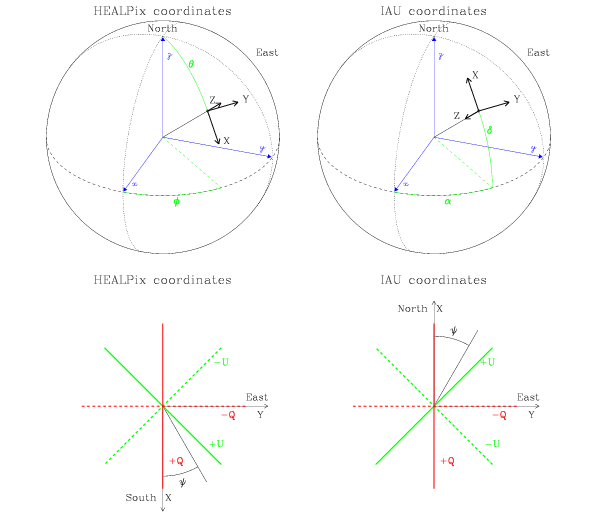
\includegraphics[bb=1pt 1pt 600pt 520pt,clip,width=0.99\textwidth,clip]{fig/merge_reftqu}\htmlimage{}}
\par

\end{figure}%
\lthtmlfigureZ
\lthtmlcheckvsize\clearpage}

\stepcounter{subsection}
{\newpage\clearpage
\lthtmldisplayA{eqnarray578}%
\begin{eqnarray}
	Y_{lm}(\theta,\phi) &=& \lambda_{lm}(\cos\theta) {\rm { e}}^{{i}
	m\phi} 
\htmlimage{}
\end{eqnarray}%
\lthtmldisplayZ
\lthtmlcheckvsize\clearpage}

{\newpage\clearpage
\lthtmldisplayA{eqnarray586}%
\begin{eqnarray}
	\lambda_{lm}(x) &=& \sqrt{ \frac{2l+1}{4\pi}
	\frac{(l-m)!}{(l+m)!} } P_{lm}(x), \quad{\rm for~}
	m\ge 0 	
\\
\lambda_{lm} &=& (-1)^m \lambda_{l|m|}, \quad{\rm for~}
	m <  0, \nonumber \\
\lambda_{lm} &=& 0, \quad{\rm for}\, |m| > l.\nonumber
	\htmlimage{}
\end{eqnarray}%
\lthtmldisplayZ
\lthtmlcheckvsize\clearpage}

{\newpage\clearpage
\lthtmlinlinemathA{tex2html_wrap_inline1479}%
$x\equiv\cos\theta$%
\lthtmlinlinemathZ
\lthtmlcheckvsize\clearpage}

{\newpage\clearpage
\lthtmldisplayA{eqnarray603}%
\begin{eqnarray}
	(1-x^2)\frac{d^2}{dx^2}P_{lm} - 2x \frac{d}{dx}P_{lm}
	+ \left(l(l+1) - \frac{m^2}{1-x^2}\right) P_{lm} &=& 0.
	\htmlimage{}
\end{eqnarray}%
\lthtmldisplayZ
\lthtmlcheckvsize\clearpage}

{\newpage\clearpage
\lthtmldisplayA{eqnarray616}%
\begin{eqnarray}
	P_{lm} &=& (-1)^m (1-x^2)^{m/2} \frac{d^m}{dx^m} P_{l}(x),
	\htmlimage{}
\end{eqnarray}%
\lthtmldisplayZ
\lthtmlcheckvsize\clearpage}

{\newpage\clearpage
\lthtmldisplayA{eqnarray625}%
\begin{eqnarray}
	P_{l}(x) &=& \frac{1}{2^ll!}\frac{d^l}{dx^l} (x^2-1)^l.
	\htmlimage{}
\end{eqnarray}%
\lthtmldisplayZ
\lthtmlcheckvsize\clearpage}

\stepcounter{section}

%
\providecommand{\npix}{{N_{\rm pix}}}%


%
\providecommand{\Opix}{{\Omega_{\rm pix}}}%


%
\providecommand{\nside}{{N_{\rm side}}}%


\renewcommand{\u}{{\bf{u}}}
{\newpage\clearpage
\lthtmlinlinemathA{tex2html_wrap_inline1495}%
${\Omega_{\rm pix}}$%
\lthtmlinlinemathZ
\lthtmlcheckvsize\clearpage}

{\newpage\clearpage
\lthtmldisplayA{eqnarray646}%
\begin{eqnarray}
  f(p) &=& \int d\u w_p(\u )f(\u ) \htmlimage{}
\end{eqnarray}%
\lthtmldisplayZ
\lthtmlcheckvsize\clearpage}

{\newpage\clearpage
\lthtmlinlinemathA{tex2html_wrap_inline1499}%
$1/{\Omega_{\rm pix}}$%
\lthtmlinlinemathZ
\lthtmlcheckvsize\clearpage}

{\newpage\clearpage
\lthtmlinlinemathA{tex2html_wrap_inline1501}%
$\int d\u w_p(\u ) = 1$%
\lthtmlinlinemathZ
\lthtmlcheckvsize\clearpage}

{\newpage\clearpage
\lthtmldisplayA{eqnarray650}%
\begin{eqnarray}
  f(p)&=&\sum_{l=0}^{l_{max}}\sum_{m}a_{lm}w_{lm}(p),
\htmlimage{}
\end{eqnarray}%
\lthtmldisplayZ
\lthtmlcheckvsize\clearpage}

{\newpage\clearpage
\lthtmldisplayA{eqnarray658}%
\begin{eqnarray}
 	w_{lm}(p) &=& \int d\u w_p(\u ) Y_{lm}(\u ), \htmlimage{} 
\end{eqnarray}%
\lthtmldisplayZ
\lthtmlcheckvsize\clearpage}

{\newpage\clearpage
\lthtmldisplayA{eqnarray666}%
\begin{eqnarray}
  w_{lm}(p) = w_l(p) Y_{lm}(p)\htmlimage{}
\end{eqnarray}%
\lthtmldisplayZ
\lthtmlcheckvsize\clearpage}

{\newpage\clearpage
\lthtmldisplayA{eqnarray671}%
\begin{eqnarray}
	w_{l}(p) &=& \left(\frac{4 \pi}{2l+1}\sum_{m=-l}^{l} \left|w_{lm}(p)\right|^2\right)^{1/2},\htmlimage{}
	
\end{eqnarray}%
\lthtmldisplayZ
\lthtmlcheckvsize\clearpage}

{\newpage\clearpage
\lthtmlinlinemathA{tex2html_wrap_inline1509}%
$C_{l}^{\rm pix}$%
\lthtmlinlinemathZ
\lthtmlcheckvsize\clearpage}

{\newpage\clearpage
\lthtmlinlinemathA{tex2html_wrap_inline1511}%
$C_{l}^{\rm unpix}$%
\lthtmlinlinemathZ
\lthtmlcheckvsize\clearpage}

{\newpage\clearpage
\lthtmldisplayA{eqnarray686}%
\begin{eqnarray}
	C_{l}^{\rm pix} &=& w^2_{l} C_{l}^{\rm unpix} \htmlimage{}
	
\end{eqnarray}%
\lthtmldisplayZ
\lthtmlcheckvsize\clearpage}

{\newpage\clearpage
\lthtmldisplayA{eqnarray696}%
\begin{eqnarray}
	w_{l} &=& \left(\frac{1}{{N_{\rm pix}}}\sum_{p=0}^{{N_{\rm pix}}-1} w^2_{l}(p)\right)^{1/2}.\htmlimage{}
	
\end{eqnarray}%
\lthtmldisplayZ
\lthtmlcheckvsize\clearpage}

{\newpage\clearpage
\lthtmlinlinemathA{tex2html_wrap_inline1515}%
$l\le 4{N_{\rm side}}$%
\lthtmlinlinemathZ
\lthtmlcheckvsize\clearpage}

{\newpage\clearpage
\lthtmlinlinemathA{tex2html_wrap_inline1517}%
${N_{\rm side}}$%
\lthtmlinlinemathZ
\lthtmlcheckvsize\clearpage}

{\newpage\clearpage
\lthtmlinlinemathA{tex2html_wrap_inline1519}%
${N_{\rm side}}\le 128$%
\lthtmlinlinemathZ
\lthtmlcheckvsize\clearpage}

{\newpage\clearpage
\lthtmlinlinemathA{tex2html_wrap_inline1521}%
${N_{\rm side}}> 128$%
\lthtmlinlinemathZ
\lthtmlcheckvsize\clearpage}

{\newpage\clearpage
\lthtmlinlinemathA{tex2html_wrap_inline1525}%
${N_{\rm side}}= 128$%
\lthtmlinlinemathZ
\lthtmlcheckvsize\clearpage}

{\newpage\clearpage
\lthtmlinlinemathA{tex2html_wrap_inline1539}%
$\Delta w/w < 7\ 10^{-4}$%
\lthtmlinlinemathZ
\lthtmlcheckvsize\clearpage}

{\newpage\clearpage
\lthtmlinlinemathA{tex2html_wrap_inline1541}%
$l=2{N_{\rm side}}$%
\lthtmlinlinemathZ
\lthtmlcheckvsize\clearpage}

{\newpage\clearpage
\lthtmlinlinemathA{tex2html_wrap_inline1543}%
$\Delta w/w < 1.7\ 10^{-3}$%
\lthtmlinlinemathZ
\lthtmlcheckvsize\clearpage}

{\newpage\clearpage
\lthtmlinlinemathA{tex2html_wrap_inline1545}%
$l=4{N_{\rm side}}$%
\lthtmlinlinemathZ
\lthtmlcheckvsize\clearpage}

\stepcounter{section}
{\newpage\clearpage
\lthtmlinlinemathA{tex2html_wrap_inline1549}%
$x\in]0,1[$%
\lthtmlinlinemathZ
\lthtmlcheckvsize\clearpage}

{\newpage\clearpage
\lthtmlinlinemathA{tex2html_wrap_inline1551}%
$2^{128}-1 \approx 3.4 10^{38}$%
\lthtmlinlinemathZ
\lthtmlcheckvsize\clearpage}

{\newpage\clearpage
\lthtmlinlinemathA{tex2html_wrap_inline1553}%
$\hat{{\rm a}}$%
\lthtmlinlinemathZ
\lthtmlcheckvsize\clearpage}


\end{document}
